\section{Introduction}

This document describes client requirements and system 
requirements for a SQUID magnetometer program that will be designed and 
implemeted as a software engineering student project at University of 
Helsinki at the Computer Science Department. The client is the Department 
of Geophysics.

This document serves as a contract between client and us..

Expected readership of this document here..

\subsection{Glossary}

Technical terms here..

\section{Overview}

A brief overview of the problem domain..


\section{Use cases}

% super-makrot uce caseille
\newcommand{\uctitle}[1]{\stepcounter{ucnum}\textbf{UC\arabic{ucnum}: #1}\\}
\newcommand{\ucscenario}[1]{\stepcounter{ucsce}\textbf{Scenario \alph{ucsce}:} #1\\}
\newcommand{\ucpre}[1]{\textbf{Precondition:} #1\\}
\newcommand{\ucpost}[1]{\textbf{Postcondition:} #1\\}
\newcommand{\ucerror}[1]{\textbf{Error condition:} #1\\}
\newcounter{ucnum}
\newcounter{ucsce}[ucnum]

Describes planned use cases for the program. Derived from user interface prototype and user requiremets. All use cases are made by "the user" in program main screen, unless otherwise noted.

Format for uce cases:

\setcounter{ucnum}{-1}
\uctitle{Uce case number and title}
\ucscenario{First scenario for doing the use case}
\ucscenario{Second scenario for doing the use case}
\ucpre{Preconditions for use case}
\ucpost{Postconditions for use case}
\ucerror{Error handling, mainly if anything special needs to be done}


\subsection{Measuring}

\uctitle{Do single step measuring without demagnetization}
\ucscenario{Enter as next AF demagnetization step "0" or empty (default for new projects), meaning no demagnetization, and click "Single step".}
\ucpre{Open AF project, sample in sample holder.}
\ucpost{Sample measured, results on screen.}
\ucerror{The program shall let the user know if something went wrong.}

\uctitle{Do single step measuring with demagnetization}
\ucscenario{Enter as next AF demag step anything greater than zero, and click "Single step".}
\ucpre{Open AF project, sample in sample holder.}
\ucpost{Sample demagnetized (possibly ruined) and measured, results on screen.}
\ucerror{The program shall let the user know if something went wrong, and, should the demagnetization field not be coming down, warn user with an alarm sound :)}

\uctitle{Do automatic demagnetization-measuring sequence}
\ucscenario{Enter the AF sequence (see \ref{sequsecaseaf} for ways to enter it) and click "Measure".}
\ucpre{Open AF project, sample in sample holder.}
\ucpost{Sample demagnetized according to entered AF sequence (possibly ruined) and measured after each demagnetization, results on screen.}
\ucerror{The program shall let the user know if something went wrong, and, should the demagnetization field be uncalm, warn user with an alarm sound x)}

  \uctitle{Pause automatic measuring sequence}
  \ucscenario{While measure sequence is running, click "Pause".}
  \ucpre{Ongoing measure sequence.}
  \ucpost{Measure sequence halts after current step is done, results on screen.}
  \ucerror{Program tells if sequence can't be paused (and something has gone terribly wrong).}

  \uctitle{Abort automatic measuring sequence}
  \ucscenario{While measure sequence is running or paused, click "Stop immediately".}
  \ucpre{Ongoing or paused measure sequence.}
  \ucpost{Measure sequence halts immediately [and program enters "fully manual" mode?]}
  \ucerror{Program tells if sequence can't be aborted (and something has gone terribly wrong).}

\uctitle{Do thellier measuring}
\ucscenario{Click "Single step". (Temperature can be entered later, as it won't affect measuring.)}
\ucpre{Open TH project, sample in sample holder.}
\ucpost{Sample measured, results on screen.}
\ucerror{As usual.}

\uctitle{Do thermal measuring}
{}[Exactly the same as thellier?]\\
\ucscenario{Click "Single step". (Temperature can be entered later, as it won't affect measuring.)}
\ucpre{Open TH project, sample in sample holder.}
\ucpost{Sample measured, results on screen.}
\ucerror{As usual.}

\uctitle{Measure magnetometer ground noise}
{}[2005-02-23 not in current UI proto, nor planned for implementation]\\
\ucscenario{Click "Ground noise" and "Calibrate".}
\ucpre{None.}
\ucpost{Ground noise measured, results on screen.}

\uctitle{Measure empty sample holder noise}
{}[2005-02-21 In current UI prototype, "Noise" actually does sample holder noise measuring.]\\
\ucscenario{Click "Holder noise" and "Calibrate".}
\ucpre{Empty sample holder.}
\ucpost{Holder noise measured, results on screen.}

\uctitle{Fully manual measuring}
- Demagnetize X, Y or Z axis\\
- item Measure X, Y or Z axis\\
\ucscenario{Click any of the manual control components [2005-02-21 at right third of UI proto].}
\ucpre{Manual mode enabled.}
\ucpost{Manual action done, result on screen.}

\uctitle{Enable manual mode}
\ucscenario{Click "Manual" checkbox above the manual control components.}
\ucpre{No ongoing measurement.}
\ucpost{Manual mode enabled.}


\subsection{File formats}

\uctitle{Automatically save all measurement cycles in project [.dat?] file}
\ucscenario{Make any measurement action.}
\ucpre{Open project file.}
\ucpost{After measurement is done, new results appended to project file.}

\uctitle{Save standard sample measurement results in .std file}
\ucscenario{Click "Standard sample", "Calibrate".}
\ucpre{No ongoing measurement.}
\ucpost{After standard sample measurement is done, new results appended to predefined .std file.}

\uctitle{Export project data into .dat file}
\ucscenario{In project explorer file list, right-click on desired project file, click "Export .dat in current directory".}
\ucscenario{In project explorer file list, right-click on desired project file, click "Export .dat to disk drive A:".}
\ucscenario{In project explorer file list, right-click on desired project file, click "Export .dat...", chooce directory and filename to export.}
\ucpre{At least 1 project file in current (selected) directory.}
\ucpost{Project data exported to .dat file.}
\ucerror{Notify if file error occurs (such as no disk in A: drive).}

\uctitle{Export (thellier) project data into .tdt file}
\ucscenario{In project explorer file list, right-click on desired project file, click "Export .tdt in current directory".}
\ucscenario{In project explorer file list, right-click on desired project file, click "Export .tdt to disk drive A:".}
\ucscenario{In project explorer file list, right-click on desired project file, click "Export .tdt...", chooce directory and filename to export.}
\ucpre{At least 1 project file in current (selected) directory.}
\ucpost{Project data exported to .tdt file.}
\ucerror{Notify if file error occurs (such as no disk in A: drive).}

\uctitle{Export single measurement details into .srm file}
\ucscenario{In measurement result table, right-click on desired measurement line, click "Export .srm in current directory".}
\ucscenario{In measurement result table, right-click on desired measurement line, click "Export .srm to disk drive A:".}
\ucscenario{In measurement result table, right-click on desired measurement line, click "Export...", chooce directory and filename to export.}
\ucpre{At least 1 measurement result in current project.}
\ucpost{Measurement details exported to .srm file.}
\ucerror{Notify if file error occurs (such as no disk in A: drive).}

\uctitle{Print measurement results}
\ucscenario{Click "Print...", "Measurement results". [2005-02-23 propably gone in current UI prototype; implementation priority low]}
\ucpre{Open project.}
\ucpost{Measurement results printed via [Java] standard printing window.}
\ucerror{Let know if printing error occurs.}

\uctitle{Print graph sheet (with 7 different graphs; described elsewhere)}
\ucscenario{Click "Print...", "Grap sheet". [2005-02-23 propably gone in current UI prototype; implementation priority low]}
\ucpre{Open project.}
\ucpost{Measurement results printed via [Java] standard printing window.}
\ucerror{Let know if printing error occurs.}


\subsection{Functionality}

\uctitle{Create new project [.dat file?]}

\uctitle{Load project [.dat file?]}

\uctitle{Append measurement results to project [.dat file?]}

\uctitle{Panic abort operation instantly}

When any measuring action, click "Stop immediately".

\ucpre{Single step measuring or ongoing measure sequence.}
\ucpost{All demagnetization and measuring halts immediately [and program enters "fully manual" mode?]}
\ucerror{Program tells if measuring can't be aborted, meaning something has gone terribly wrong.}

\subsection{AF sequences}
\label{sequsecaseaf}

{\it As in automatic demagnetization-measuring sequences, or Alternating Field sequences}

\uctitle{Insert AF sequence with start-step-stop values}

\uctitle{Load AF sequence}

\uctitle{Save AF sequence}

\uctitle{Edit AF sequence on-the-fly}

\uctitle{Edit stored AF sequences}

\uctitle{Rename stored AF sequence}

\uctitle{Delete stored AF sequence}


\section{User requirements}

% Makrot vaatimuksille
\newcommand{\ReqId}[1]{\textbf{Identifier:} #1\\}
\newcommand{\ReqName}[1]{\textbf{Name:} #1\\}
\newcommand{\ReqDesc}[1]{\textbf{Description:} #1\\}
\newcommand{\ReqPrio}[1]{\textbf{Priority:} #1\\}

Goals of the software set by client..

\subsection{Functional requirements}

\ReqId{R1}
\ReqName{Basic}
\ReqDesc{Able to control Squid-magnetometer and make measurements with it.}
\ReqPrio{1}

\ReqId{R2}
\ReqName{Saving}
\ReqDesc{Measurements can be saved in .dat, .dtd and .srm files.}
\ReqPrio{1}

\ReqId{R3}
\ReqName{Auto saving}
\ReqDesc{Program will save mesurement data after every measurement step.}
\ReqPrio{1}

\ReqId{R4}
\ReqName{Loading}
\ReqDesc{Saved mesurement date can be loaded into program.}
\ReqPrio{2}

\ReqId{R5}
\ReqName{Filemanagement}
\ReqDesc{New data can be added to existing datafiles.}
\ReqPrio{2}

\ReqId{R6}
\ReqName{Numeric presentation of data}
\ReqDesc{Program shows measurement data in numbers.}
\ReqPrio{1}

\ReqId{R7}
\ReqName{Graphic presentation of data}
\ReqDesc{Program draws graphs from measurement data.}
\ReqPrio{3}

\ReqId{R8}
\ReqName{Editing}
\ReqDesc{Ability edit data afterwards.}
\ReqPrio{2}

\ReqId{R9}
\ReqName{Recalculation}
\ReqDesc{Recalculate based on changed data.}
\ReqPrio{2}

\ReqId{R10}
\ReqName{Control}
\ReqDesc{Ability to stop any action immediately.}
\ReqPrio{1}

\ReqId{R11}
\ReqName{Sequence}
\ReqDesc{Able to create measuring sequences with several different sized steps.}
\ReqPrio{2}

\ReqId{R12}
\ReqName{Sequence control}
\ReqDesc{Able to stop sequence after current step.}
\ReqPrio{2}

\ReqId{R13}
\ReqName{Hotkeys}
\ReqDesc{Possibility to create and change hotkeys.}
\ReqPrio{4}

\ReqId{R14}
\ReqName{Manual}
\ReqDesc{Able to operate magnetometer manually.}
\ReqPrio{2}

ReqId{R15}
\ReqName{Calibration}
\ReqDesc{Magnetometer must be calibrated every 24h..}
\ReqPrio{2}

ReqId{RXX}
\ReqName{}
\ReqDesc{}
\ReqPrio{}

\subsection{Quality requirements}

\ReqId{QR1}
\ReqName{Ease of use}
\ReqDesc{Program should be easy to use for first time users.}
\ReqPrio{1}

\ReqId{QR2}
\ReqName{Help pages}
\ReqDesc{Program should have good help pages.}
\ReqPrio{3}

\subsection{Environment}

\subsection{Maintainability}

\subsection{Restrictions}

Program will be used in normal PC which is connected to magnetometer. 
Taking into account rapid phase of computer evolution it is possible 
that computer in which program is used can change, accordingly the 
program should be able to be installed by outsiders. 
We need not prepare to changing of magnetometer, as new 
magnenetometer will probably have its own program.


\section{System requirements / Functions}

Specific explanation of the functions to be implemented

\subsection{System restrictions}

\section{User interface}

Overview of UI described here.. 

\subsection{Goal derived use cases}


\section{Architecture overview}

\begin{figure}
\begin{center}
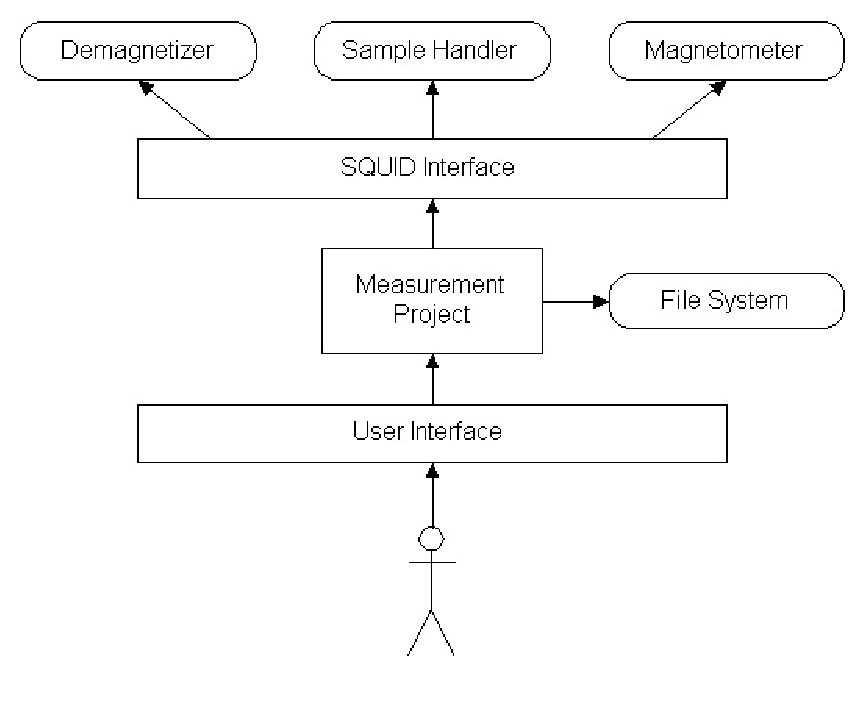
\includegraphics[width=10cm]{architecture.eps}
\caption{Architecture overview}
\label{fig:architecture}
\end{center}
\end{figure}


\section{External interfaces}

Interfaces to existing software and hardware are described here.

\subsection{Existing program}

The existing software for using the SQUID is "2G Enterprises Data Acquisition". 
We have access to the source code for version 2.99.3 of the program. From the 
old source code we will reuse basically only the SerialIO component. We will 
build an interface for communicating with the SQUID hardware by using Java and 
JNI (Java Native Interface).

\subsection{Hardware control protocols}

The SQUID consists of three independent units:

\begin{itemize}
\item Automated Sample Handler System (MODEL 2G800)
\item Automatic Sample Degaussing System (MODEL 2G600)
\item Superconducting Rock Magnetometer (MODEL 755R or 760R)
\end{itemize}

Automated Sample Handler System controls the movement and rotation of the sample 
holder. Its protocol is described in Appendix 1.

Automatic Sample Degaussing System controls the demagnetizer. Its protocol is 
described in Appendix 2.

Superconducting Rock Magnetometer reads the measurements from the magnetometer. 
Its protocol is described in Appendix 3.


\section{Validation}

Description of how to validate the set requirements.
